\documentclass{article}

\usepackage{Sweave}
\begin{document}
\input{TP1-concordance}

\title{TP1 - Recursion equation}

\maketitle

\section{Model implementation}

General function frecurs
\begin{Schunk}
\begin{Sinput}
> # n is time, u0 the initial condition, func the recursive function
> 
> frecurs <- function(show, n=0, u0, func,...) {
+   if (show) print(u0)
+   if (n==0) return(u0)
+   else return(frecurs(show = show, n=n-1, u0 = func(u0,...), func, ...))
+ }
\end{Sinput}
\end{Schunk}

\begin{Schunk}
\begin{Sinput}
> frecurs2 <- function(n=0, u0, func,...) {
+   
+   if (n==0) return(u0)
+   else return(c(u0, frecurs2(n=n-1, u0 = func(u0,...), func, ...)))
+ }
> 
\end{Sinput}
\end{Schunk}


\begin{Schunk}
\begin{Sinput}
> exponential <- function(N, r) {
+   return(r*N)
+ }
\end{Sinput}
\end{Schunk}

\begin{Schunk}
\begin{Sinput}
> logarithmic <- function(N, r, K) {
+   return(r*N*(1-(N/K)))
+ }
\end{Sinput}
\end{Schunk}

\begin{Schunk}
\begin{Sinput}
> gompertz <- function(N, r, K) {
+   return(-r*N*log(N/K))
+ }
\end{Sinput}
\end{Schunk}

\subsection{Basic verifications}
\begin{Schunk}
\begin{Sinput}
> # Exponential
> frecurs(TRUE, 50, 2, exponential, 2)
\end{Sinput}
\begin{Soutput}
[1] 2
[1] 4
[1] 8
[1] 16
[1] 32
[1] 64
[1] 128
[1] 256
[1] 512
[1] 1024
[1] 2048
[1] 4096
[1] 8192
[1] 16384
[1] 32768
[1] 65536
[1] 131072
[1] 262144
[1] 524288
[1] 1048576
[1] 2097152
[1] 4194304
[1] 8388608
[1] 16777216
[1] 33554432
[1] 67108864
[1] 134217728
[1] 268435456
[1] 536870912
[1] 1073741824
[1] 2147483648
[1] 4294967296
[1] 8589934592
[1] 17179869184
[1] 34359738368
[1] 68719476736
[1] 1.37439e+11
[1] 274877906944
[1] 549755813888
[1] 1.099512e+12
[1] 2.199023e+12
[1] 4.398047e+12
[1] 8.796093e+12
[1] 1.759219e+13
[1] 3.518437e+13
[1] 7.036874e+13
[1] 1.407375e+14
[1] 2.81475e+14
[1] 5.6295e+14
[1] 1.1259e+15
[1] 2.2518e+15
[1] 2.2518e+15
\end{Soutput}
\begin{Sinput}
> # Logarithmic
> frecurs(TRUE, 50, 2, logarithmic, 2, 10)
\end{Sinput}
\begin{Soutput}
[1] 2
[1] 3.2
[1] 4.352
[1] 4.916019
[1] 4.998589
[1] 5
[1] 5
[1] 5
[1] 5
[1] 5
[1] 5
[1] 5
[1] 5
[1] 5
[1] 5
[1] 5
[1] 5
[1] 5
[1] 5
[1] 5
[1] 5
[1] 5
[1] 5
[1] 5
[1] 5
[1] 5
[1] 5
[1] 5
[1] 5
[1] 5
[1] 5
[1] 5
[1] 5
[1] 5
[1] 5
[1] 5
[1] 5
[1] 5
[1] 5
[1] 5
[1] 5
[1] 5
[1] 5
[1] 5
[1] 5
[1] 5
[1] 5
[1] 5
[1] 5
[1] 5
[1] 5
[1] 5
\end{Soutput}
\begin{Sinput}
> # Gompertz
> frecurs(TRUE, 50, 2, gompertz, 2, 10)
\end{Sinput}
\begin{Soutput}
[1] 2
[1] 6.437752
[1] 5.670446
[1] 6.433885
[1] 5.674771
[1] 6.430139
[1] 5.678957
[1] 6.426507
[1] 5.683011
[1] 6.422983
[1] 5.68694
[1] 6.419563
[1] 5.690751
[1] 6.416241
[1] 5.694448
[1] 6.413012
[1] 5.698038
[1] 6.409873
[1] 5.701526
[1] 6.406819
[1] 5.704916
[1] 6.403846
[1] 5.708214
[1] 6.400951
[1] 5.711422
[1] 6.39813
[1] 5.714546
[1] 6.39538
[1] 5.717588
[1] 6.392699
[1] 5.720552
[1] 6.390083
[1] 5.723442
[1] 6.38753
[1] 5.72626
[1] 6.385037
[1] 5.72901
[1] 6.382602
[1] 5.731694
[1] 6.380223
[1] 5.734315
[1] 6.377897
[1] 5.736875
[1] 6.375623
[1] 5.739377
[1] 6.373399
[1] 5.741823
[1] 6.371223
[1] 5.744214
[1] 6.369093
[1] 5.746553
[1] 5.746553
\end{Soutput}
\end{Schunk}

\subsection{Stair step diagram}
\begin{Schunk}
\begin{Sinput}
> r0 = 1.5
> tmax = 50
> K0 = 10
> Ni = 2
> cobweb_diagram = function(tmax, Ni, funct, r = r0, K = K0, lim) {
+   
+   if (funct == 1) {
+       N = frecurs2(tmax, Ni, func = exponential, r = r0)
+       curve(r0*x, from=0, to = lim, las=1,
+         xlab = expression(N[t]), ylab = expression(N[t+1]), 
+         main = 'Exponential model stair step diagram', lwd = 2)
+   } else if (funct == 2) {
+       N = frecurs2(tmax, Ni, func = logarithmic, r = r0, K = K0)
+       curve(r0*x*(1-(x/K0)), from=0, to = lim, las=1,
+         xlab = expression(N[t]), ylab = expression(N[t+1]), 
+         main = 'Logistic model stair step diagram', lwd = 2)
+   } else if (funct == 3) {
+       N = frecurs2(tmax, Ni, func = gompertz, r = r0, K = K0)
+       curve(-r0*x*log(x/K0), from=0, to = lim, las=1,
+         xlab = expression(N[t]), ylab = expression(N[t+1]), 
+         main = 'Gompertz model stair step diagram', lwd = 2)
+   }
+   
+   abline(a = 0, b = 1, col = 'blue', lwd = 2)
+   abline(h = 0, lty = 3)
+   abline(v = 0, lty = 3)
+   points(N, N, type = 'S', col = 'red')
+   legend('topright', c('f(n)', expression (paste(paste(n[t+1], '='), n[t])), 'stair steps'), 
+        lty = 1, col = c('black', 'blue', 'red'), lwd = 2)
+ }
> cobweb_diagram(tmax, Ni, 1, r = r0, lim = 30)
> cobweb_diagram(tmax, Ni, 2, r = r0, K0, 10)
> cobweb_diagram(tmax, Ni, 3, r = r0, K0, 10)
\end{Sinput}
\end{Schunk}
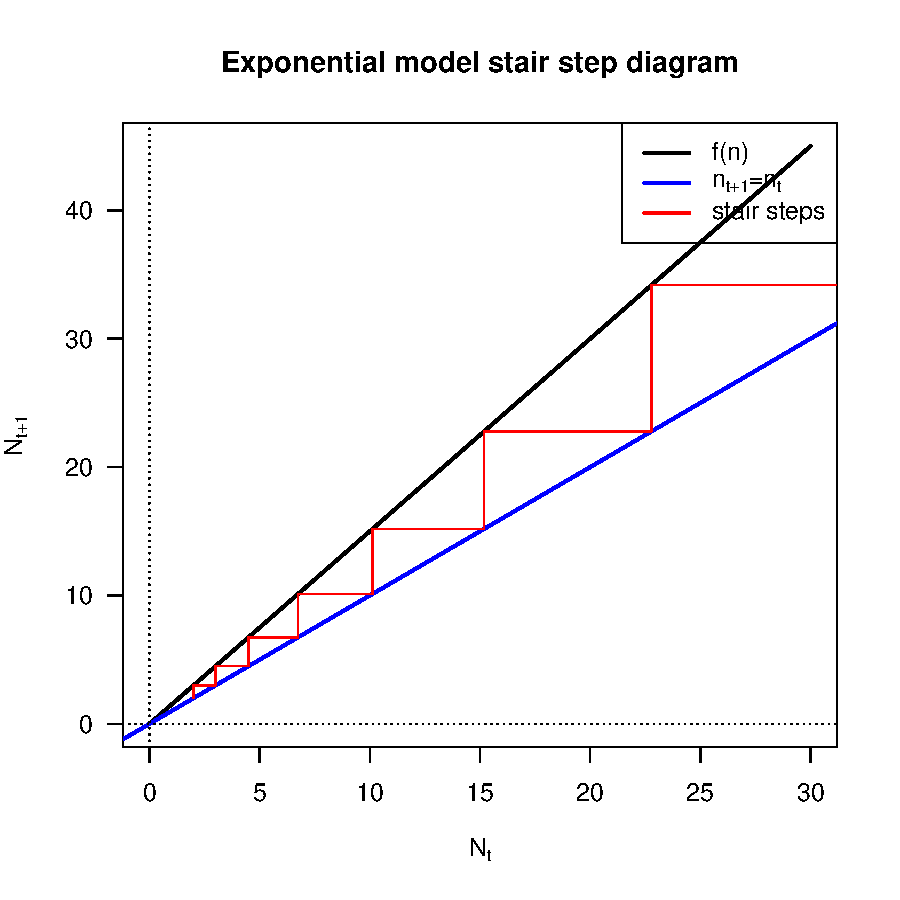
\includegraphics{TP1-007}

\begin{Schunk}
\begin{Sinput}
> t = seq(0,50)
> par(mfrow = c(2,2))
> for (i in c(1.5, 2.8, 3.1, 3.7)) {
+   plot(t, frecurs2(tmax, 10, func = exponential, r = i), main = paste('r =', i))
+ }
\end{Sinput}
\end{Schunk}
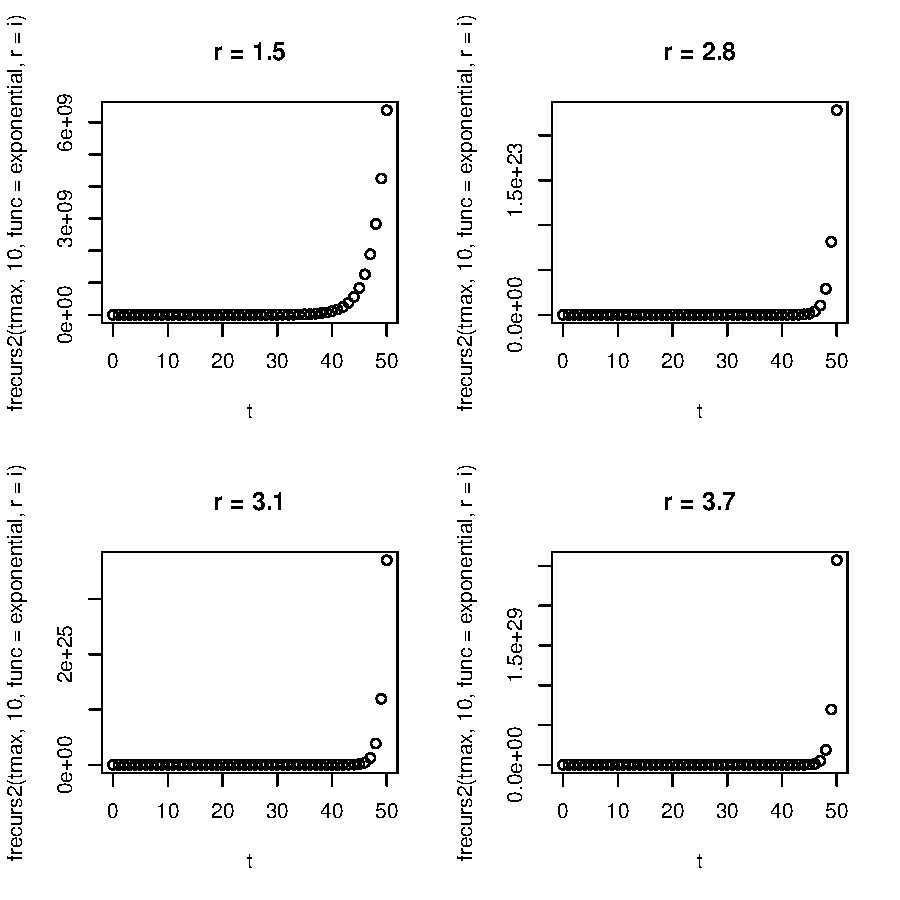
\includegraphics{TP1-008}

\begin{Schunk}
\begin{Sinput}
> par(mfrow = c(2,2))
> for (i in c(1.5, 2.8, 3.1, 3.7)) {
+   plot(t, frecurs2(tmax, 10, func = logarithmic, r = i, K = 1000), main = paste('r =', i))
+ }
\end{Sinput}
\end{Schunk}
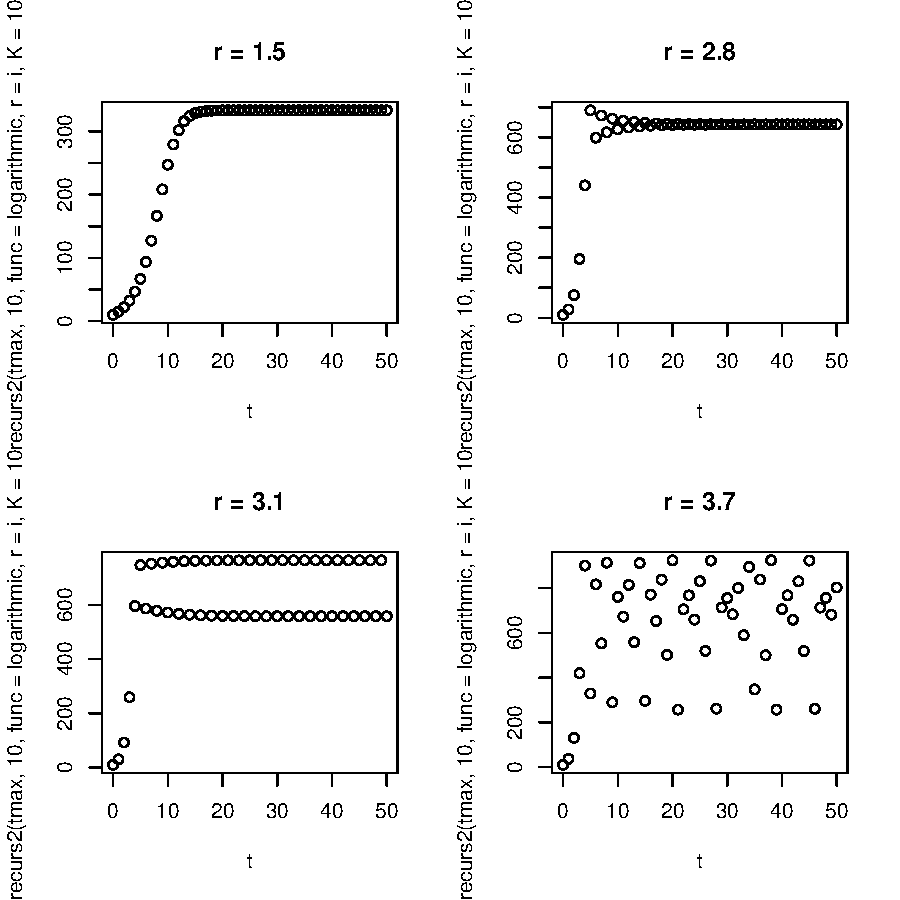
\includegraphics{TP1-009}

\begin{Schunk}
\begin{Sinput}
> par(mfrow = c(2,2))
> for (i in c(1.5, 2.8, 3.1, 3.7)) {
+   plot(t, frecurs2(tmax, 10, func = gompertz, r = i, K = 1000), main = paste('r =', i))
+ }
\end{Sinput}
\end{Schunk}
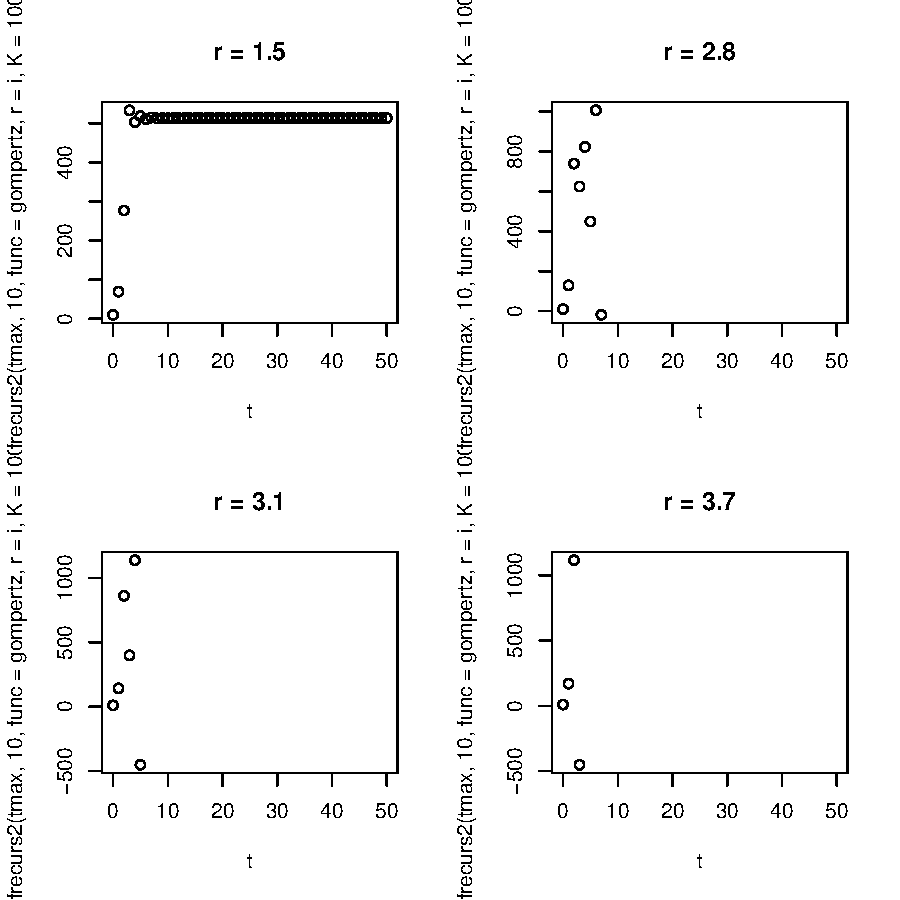
\includegraphics{TP1-010}

\subsection{Bifurcation diagram}

\begin{Schunk}
\begin{Sinput}
> par(mfrow = c(1,1))
> plot(0, xlim = c(3,4), ylim = c(0,200), cex = 0.01)
> for (i in seq(0,4,0.01)) {
+   points(rep(i, 4002), frecurs2(500, 10, func = logarithmic, r = i, K = 200)[100:501], cex = 0.01)
+ }